\documentclass[a4paper,12pt,english]{article}
\usepackage[nottoc,numbib]{tocbibind}
\usepackage[utf8]{inputenc}
\usepackage[english]{babel}
\usepackage{amsmath}
\usepackage{amssymb}
\usepackage{listings}
\usepackage{hyperref}
\usepackage{booktabs}
\usepackage{graphicx}
\usepackage{makeidx}
\usepackage{titlesec}
\usepackage{fancyhdr}
\usepackage{wrapfig}
\usepackage{fancyvrb}
\usepackage{pbox}
\usepackage{hyperref}
\usepackage{mathtools}
\usepackage{amsmath}
\usepackage{multicol}
\usepackage{tocloft}%
\usepackage[refpage]{nomencl}
\usepackage{etoolbox}
\apptocmd{\sloppy}{\hbadness 10000\relax}{}{}
\makenomenclature

\graphicspath{ {/} }
\pagestyle{fancy}
\setcounter{secnumdepth}{3}
\setcounter{tocdepth}{3}

%Setting link borders to none
\hypersetup{pdfborder = {0 0 0}}

\fancyhead[C]{}
\fancyhead[L]{}
\fancyhead[R]{\footnotesize{
Sebastian O. Jensen}}


\begin{document}
\pagenumbering{Alph}
\begin{titlepage}

\newcommand{\HRule}{\rule{\linewidth}{0.4mm}}
\center
\small{ \emph{Forfattere:}\\
14.06-79 Sebastian O. Jensen \textsc{GJX653}
\\
Hold 1} \\[2cm]

\textsc{\LARGE Fotonik}\\[0.5cm]
\textsc{\large DTU}\\[1.5cm]
\textsc{\huge Protocols and standards in IoT}\\
\HRule \\[0.7cm]
{\bfseries Keywords: ZigBee, Mesh networking, IEEE 802.15.4, MQTT-SN,
TI CC2530, IAR Workbench, Nodejs, MongoDB, FlipDots, Raspberry pi,
REST}\\[0.4cm]
\HRule
\\[1.5cm] \textsc{\Large \textsc{\today}}\\[0.5cm]



\end{titlepage}

\tableofcontents

\pagenumbering{arabic}
\section{Introduction}	
\subsection{Abstract}
Forecasts say that in 2020 there will be 25 Billion devices connected to the
internet. In 2014 it was estimated to be 3.7 Billion devices\cite{Gartner}.
This put a big demand on common tehnologies such as wifi, http, relational
databases, etc. This project investigate how to deal with these challenges by
building a prototype of a system that meets these challenges. The system
consist of multiple devices which connect in a local network and are made
availerble via the internet. This is a fully realistic example of how to deal
with the futura of IoT\nomenclature{IoT}{Internet of Things}. The
application consist of some battery powered devices that communicate wireless
via the ZigBee protocol, a ZigBee/internet gateway and an application server
where the backend, a database and a webportal is implemented. This report will
focus on the devices, ZigBee protocol, gateway and communication between the
gateway and application server. The report will losely touch the design of the
application server.

\subsection{Overview of this report}
In section 1.3 is the bacground for the system described. Section 2 will give a
Theoretical background on some of the technologies which will be used
to implement the system. Section 3 will give a technical description on the
implementation of the system and section 4 contains the conclution. I is
sugested to read 
\subsection{Background}
Internet of Things is the term that describes networks of physical devices that
are connected to the internet. This can be anything like sensors, whearabels,
fridges, heating systems, lightballs and what ever you else could imagine. As
mentioned there is a high growth in the number of these devices. This project
is about solving a common problem in lesure harbours. 
In leisure, harbors there are a limited number of moorings. Therefor each boat
owner has his own mooring space. At each mooring space there are a sign which
can be set to red or green. When the owner leave the harbor he should set the
sign to green indicating that the mooring is free to use for guests. If he is
away for less than a day he can set it to red indicating that the mooring is
not free to use. When the owner returns home after some days he call the harbor
master who then flip the sign to red indicating that the mooring is no longer
free. A common problem is that the boat owners often don’t set the signs to
green when they leave the harbor. The reason is it is easier to let it stay red
instead of calling the harbor master when returning home. This often result in
many unused moorings has red signs and make it difficult for guests to find
free moorings. Another problem is the time the harbor master use on flipping
the signs for people returning home to their berth.
To solve these problems a system of electronically controlled signs is
suggested. For more details about the sugested system refer to section 3.1


{\clearpage
\subsection{Abbreviations}
\renewcommand\thepage{}
\renewcommand{\nomname}{}
\renewcommand{\pagedeclaration}[1]{}
\pagestyle{empty}
\printnomenclature[3cm]
\clearpage}



\section{Theroretical background}
\subsection{Wireless networks}
Their exist many different wireless communication standards today all serving
different purpose. There is the IEEE 802.11 specifications which define
different protocols used for implementing WLAN which we mostly use for
connecting our computers and smartphone to the internet. Then there are the
mobile networks such as GSM, EDGE, UMTS, HSPA, etc. Which are used by phones to
send voice or internet data. Some less know technollogies include AIS
\nomenclature{AIS}{Automatic Identification System} which is used to transfer
data between commercial ships over VHF and satelite. They all have different
purpose and theirfore also different demands. Eg. When handling voice calls
over the mobile network the latency should not be to high and the protocol
should suport the devices in using as litle power as posible. Here follow a list
of important factors to consider when choosing a wireless tecnology.
\begin{itemize}
  \item Bandwide
  \item Latency
  \item Power consumtion
  \item Maximum number of nodes in the network
  \item Range
  \item Reliability
  \item Cost
  \item interoparebility 
\end{itemize}

For the purpose of this project we will later in the report argue that the
ZigBee Standard is a good solution for communicating with the signs in the
harbour.

\subsection{ZigBee}
\subsubsection{Overview}
ZigBee is a standard used to connect devices. It is managed by the ZigBee
allianze which count mebers such as Texas Instruments, Philips, Silicon
Labs, NXP, Samsung and many more. ZigBee aims at being relierble, secure,
lowpower and easy for the consumer to use. ZigBee specify all the layers
in the OSI-model\nomenclature{OSI-model}{Open System Interconnection Reference
Model} 
\subsubsection{Layers}
\paragraph{Overview of the layers}
ZigBee is build on top of the 802.15.4 standard which define the PHY and MAC
layer. Therefore these layers are not defined by but implemented by
ZigBee.
On top of 802.15.4 ZigBee define the layers all the way up to and including
the APL. The layers communicate via Service Access Points
(SAP)\nomenclature{SAP}{Service Access Point}. An overview of the ZigBee
model and the SAP that makes the services availerble between
them are shown in figure from the ZigBee Alliance in fig. 1. below.
\begin{figure}[h]
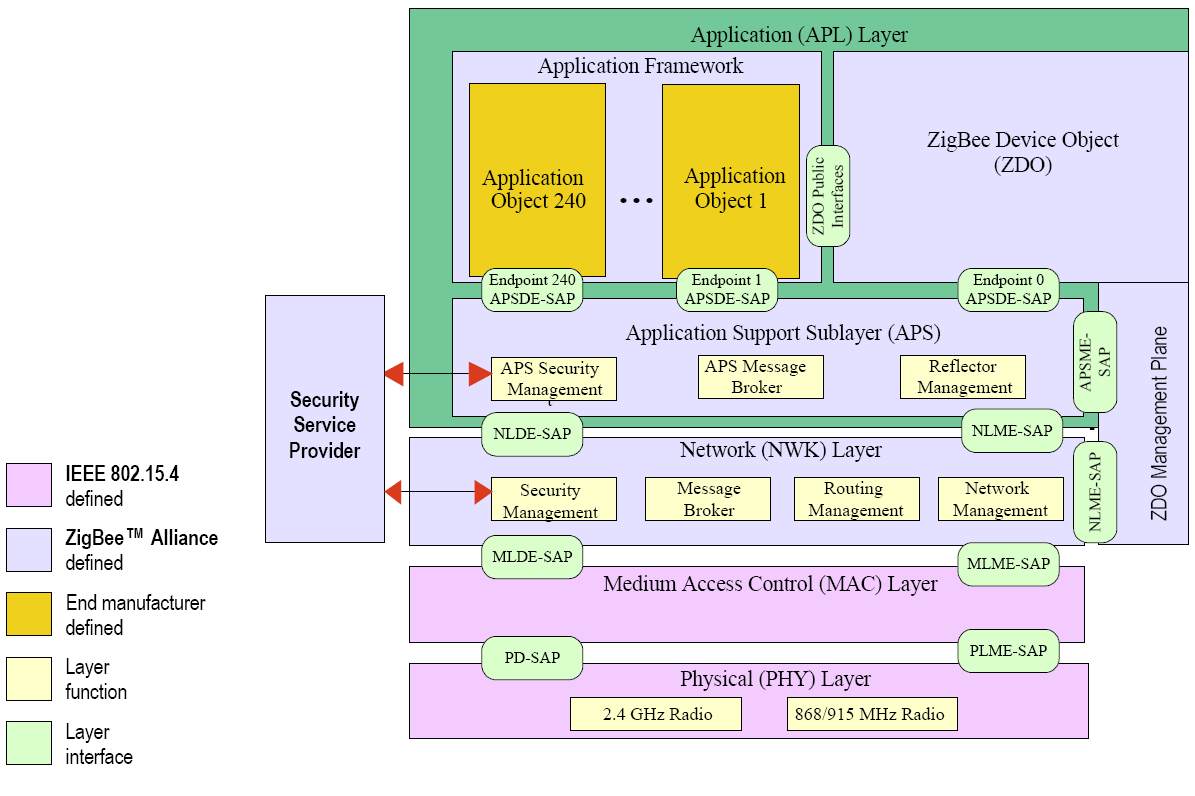
\includegraphics[width=\textwidth]{zigbeeLayers.png}
\caption{ZigBee Model\cite{zigbeeModel}}
\end{figure}

\paragraph{802.15.4}
The 802.15.4 standard specify the 2 lowest layers PHY and MAC. 802.15.4 does
specifie roles of devices, but does not implement mesh or star networking
torpology. Therefore are these funtionalities implemented by ZigBee at the
higher layers. 
\subparagraph{Physical (PHY)\nomenclature{PHY}{Physical Layer}}
The PHY is responsible for the physical part of the network. This is
harware specific things like frequency, modulation, how to avoid coalition
with other devices, receiver sensitivity, output power and other hardware
specific parametters. The PHY provide service to the MAC layer via the
PLME-SAP \nomenclature{PLME-SAP}{Physical Layer Management Entity Service Access
Point}
\subparagraph{Medium Access Layer (MAC)\nomenclature{MAC}{Medium Access Layer}}
\paragraph{Network Layer (NWK)\nomenclature{NWK}{Network Layer}}
\paragraph{Application layer\nomenclature{APL}{Aplication Layer}}
\subparagraph{Application Framework}
\subparagraph{Application Support Layer (APS)\nomenclature{APS}{Application
Support Layer}} \subparagraph{ZigBee Device Object
(ZDO)\nomenclature{ZDO}{ZigBee Device Object}}
\subsubsection{ZigBee versus other technologies}
ZigBee is not a high speed network. The maximum speed that can be
achived on the ZigBee PRO standard is 250kbit/s on 2.4Ghz, 40kbit/s on 915Mhz and 20kbit/s on868Mhz which are the 3 bands the ZigBee can
use\cite{zigbee}.
This is not much compared with the latest public wlan standard 802.11ac which manage a data rate
of up to some feew Ghz depending on the configuration \cite{802.11ac}.other
standard which is worth mention in comparsion with ZigBee is bluetooth low
energy and Z-wave. A litle more on those tech

\subsection{Database system}
\subsubsection{The traditional SQL database}
\subsubsection{NoSQL databse}
\subsubsection{NoSQL versus SQL}

\section{Design of the harbour system}
\subsection{Requirements}
The functional requerments of the system requirements is as follow

\begin{itemize}
	\item The signs should automatically turn green when a boat leaves the mooring
	\item The signs should be operated from a remote plateform. E.g. a web platform
	\item The signs should be wireless controlled and battery powered as it is
	      complicated and expencive to do cabling in the harbors.
	\item Each sign should be able to hold power for minimum of 7 years.
\end{itemize}

There are
many possibilities for adding functionality to the system such as setting a
predefined time when a sign should flip and let guest see which moorings is
free and for how long. But these functionalities should be implemented on the
server side and is therefore not considered important for this project as the
focus is on the wireless communication between the signs, interconnection with the web
platform/application server. The sensor which should sense if there is a boat
at the mooring is simulated by a switch and the red green indication is
simulated with an led. Again this is do to keeping the focus around the
communication between devices and application server.

\subsection{Acrhitecture}

\subsection{Harware}
\subsubsection{Texas Instruments CC2530 SoC}
\subsubsection{FlipDots}
\subsubsection{Raspbarry Pi}
\subsubsection{Aplication server}

\subsection{Implementaision}
\subsubsection{CC2530}
	\paragraph{Z-Stack}
	\paragraph{IAR}
	\paragraph{ZNP}

\subsubsection{Raspberry Pi}
\paragraph{Linux}
\paragraph{BCM2835 Driver}
\paragraph{REST}
\paragraph{Gateway implementation}

\subsubsection{Application Server}
\paragraph{Amazon EC2}
\paragraph{Nodejs}
\paragraph{MongoDB}
\paragraph{RESTfull API}
\paragraph{Websocket}

\section{Conclusion}

\begin{itemize}
  \item{unit\_test\_heap\_initialize}
    \\
    This tests returns \textbf{passed}.
\end{itemize}

\clearpage
\begin{thebibliography}{9}


\bibitem{Gartner}
  Gartner,
  \emph{ An American information technology research and advisory
  firm}, \url{http://www.gartner.com/newsroom/id/2905717}

\bibitem{zigbeeModel}
ZigBee Alliance,
\emph{ZigBee Security, Robert Cragie},
\url{https://docs.zigbee.org/zigbee-docs/dcn/09-5378.pdf}

\bibitem{zigbee}
ZigBee Alliance,
\emph{ZigBee Pro, Technical Summary},
\url{http://www.zigbee.org/zigbee-for-developers/network-specifications/zigbeepro/}

\bibitem{802.11ac}
802.11ac A Survival Guide,
\emph{Matthew S. Gast}

\end{thebibliography}
\end{document}

